<<<<<<< HEAD
\subsection{thread access with offset}
Using an offset instead of a stride should also lead to underutilization of the cache, but not
in a way that is as dramatic as using a stride. Only sometimes could the boundary of a cache line be crossed and an
extra cache line would have to be fetched from memory. E.g. with a warp size of 32 and 4 bytes per element, one
warp would pull 1 full cache line of 128 bytes. With an offset of 1, this would no longer be the case, an extra cache line
would have to be pulled from memory. Again, our results are mixed. We see a large drop off in memory for small offsets, but this recovers
around an offset of 12 back to the value of the coalesced memory access speed. Again, this could be due to a too small data size used here, or
due to a coding mistake. This is shown in figure \ref{fig:2.4}.

\begin{figure}
    \centering
    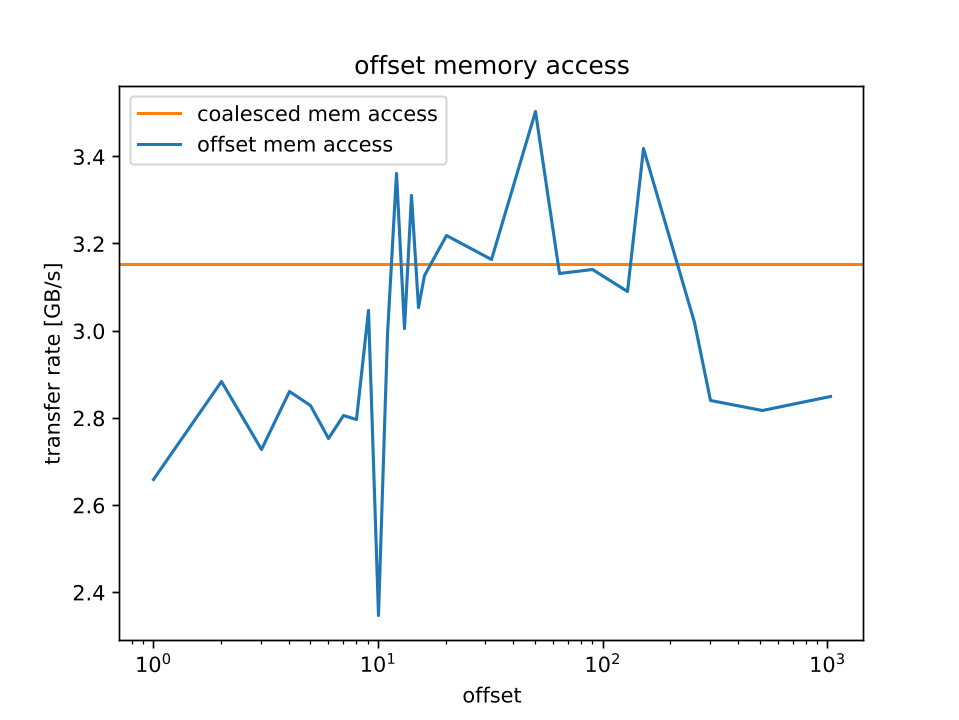
\includegraphics[scale=0.7]{pictures/offset_thread_access.png}
    \caption{exercise 3.4, thread access with offset}
    \label{fig:2.4}
\end{figure}
=======
\subsection{Global Memory -thread access with offset}
>>>>>>> 792f72f665a582f24594403cf1deafa1b2bb9d66
